%% =======================================================
%% Actividad 11: Explorando distribuciones continuas
%%
%% Compilar desde actividades/: ./compilar.sh act11
%% Las figuras de img/ se generan con: python act11.py
%% =======================================================

%% ---- CONFIGURACIÓN ------------------------

\documentclass[11pt,letterpaper]{article}

\usepackage[indice]{tecnm}
\usepackage[T1]{fontenc}
\usepackage{amsmath}
\usepackage{xcolor}
\usepackage[most]{tcolorbox} % Carga tcolorbox con soporte para listings y saltos de página
\tcbuselibrary{listings, skins, breakable}
\setlength{\emergencystretch}{3em} % Evita líneas desbordadas por palabras en \texttt

% Paleta de colores (estilo GitHub Light / VS Code)
\definecolor{codebg}{HTML}{F8F9FA}       % Fondo del código
\definecolor{codehead}{HTML}{E9ECEF}     % Fondo de la barra de título
\definecolor{codeborder}{HTML}{CED4DA}   % Borde de la tarjeta
\definecolor{codetitle}{HTML}{212529}    % Texto del título
\definecolor{codekw}{HTML}{0550AE}       % Palabras clave (import, def, for...)
\definecolor{codefunc}{HTML}{8250DF}     % Funciones y métodos (describe, groupby...)
\definecolor{codestr}{HTML}{0A3069}      % Strings
\definecolor{codecomm}{HTML}{6E7781}     % Comentarios
\definecolor{codenum}{HTML}{8C959F}      % Números de línea
\definecolor{codeid}{HTML}{24292F}       % Texto general

% Configuración base de listings
\lstdefinestyle{pythonestilo}{
  language=Python,
  basicstyle=\ttfamily\footnotesize\color{codeid},
  keywordstyle=\color{codekw}\bfseries,
  keywordstyle=[2]\color{codefunc}, % Estilo secundario para métodos de datos
  stringstyle=\color{teal!80!black},
  commentstyle=\color{codecomm}\itshape,
  morekeywords={as, True, False, None, with, yield, lambda},
  morekeywords=[2]{print, len, sum, max, DataFrame, Series, value_counts, reindex, mean, std, var, randint, normal, seed, cumsum, poisson, binom, pmf, norm, fit, kde, bincount, linspace, train_test_split, make_blobs, GaussianNB, chisquare, pdf, cdf, hist, bar, plot, axhline, axvline, fill_between, subplots, figure, concat, nunique, load_iris, diff, sort, unique},
  numbers=left,
  numberstyle=\tiny\ttfamily\color{codenum},
  stepnumber=1,
  numbersep=10pt,
  showstringspaces=false,
  morestring=[b]{"""},
  tabsize=4,
  breaklines=true,
  breakatwhitespace=true,
  columns=flexible,
  keepspaces=true,
  literate=
    {á}{{\'a}}1 {é}{{\'e}}1 {í}{{\'i}}1 {ó}{{\'o}}1 {ú}{{\'u}}1
    {Á}{{\'A}}1 {É}{{\'E}}1 {Í}{{\'I}}1 {Ó}{{\'O}}1 {Ú}{{\'U}}1
    {ñ}{{\~n}}1 {Ñ}{{\~N}}1 {¿}{{?`}}1 {¡}{{!`}}1 {°}{{$^\circ$}}1
}

% Definición del entorno personalizado \begin{codigo}{Título}{etiqueta}
% \newtcblisting[auto counter, number within=section]{codigo}[2][]{
\newtcblisting[auto counter]{codigo}[2][]{
  listing only,
  breakable,                    % Permite que el bloque se divida si pasa de página
  enhanced,
  colback=codebg,
  colframe=codeborder,
  colbacktitle=codehead,
  coltitle=codetitle,
  fonttitle=\bfseries\small\sffamily,
  boxrule=0.6pt,
  arc=4pt,                      % Bordes redondeados
  left=20pt,                    % Espacio izquierdo para los números de línea
  right=8pt,
  top=6pt,
  bottom=6pt,
  toptitle=4pt,
  bottomtitle=4pt,
  before skip=12pt,
  after skip=12pt,
  listing options={style=pythonestilo},
  title={Código \thetcbcounter: #2},
  #1
}

% Paleta para salida de consola (estilo terminal limpia)
\definecolor{termbg}{HTML}{212529}      % Fondo oscuro tipo terminal
\definecolor{termhead}{HTML}{343A40}    % Barra superior
\definecolor{termtext}{HTML}{F8F9FA}    % Texto claro de alta legibilidad
\definecolor{termborder}{HTML}{495057}  % Borde

% Entorno \begin{consola}[label=out:iris]{Título}
\newtcblisting[auto counter]{consola}[2][]{
  listing only,
  breakable,
  colback=termbg,
  colframe=termborder,
  colbacktitle=termhead,
  coltitle=termtext,
  colupper=termtext,
  fonttitle=\bfseries\small\sffamily,
  boxrule=0.6pt,
  arc=4pt,
  left=8pt,
  right=8pt,
  top=6pt,
  bottom=6pt,
  toptitle=4pt,
  bottomtitle=4pt,
  before skip=12pt,
  after skip=12pt,
  listing options={
    basicstyle=\ttfamily\scriptsize\color{termtext}, % \scriptsize evita que las tablas de Pandas se partan de línea
    breaklines=true,
    columns=fixed,        % Mantiene alineadas las columnas de Pandas
    keepspaces=true,
    showstringspaces=false,
    literate=
      {á}{{\'a}}1 {é}{{\'e}}1 {í}{{\'i}}1 {ó}{{\'o}}1 {ú}{{\'u}}1
      {Á}{{\'A}}1 {É}{{\'E}}1 {Í}{{\'I}}1 {Ó}{{\'O}}1 {Ú}{{\'U}}1
      {ñ}{{\~n}}1 {Ñ}{{\~N}}1 {°}{{$^\circ$}}1
  },
  title={Salida \thetcbcounter: #2},
  #1
}

%% ---- DATOS DE LA MATERIA ------------------------

\materia{Modelos Estadísticos para el Aprendizaje \\ Automático y Ciencia de Datos}
\actividad{Tema 2.2
Distribuciones de Probabilidad Discretas y Continuas \\ Actividad 11 - Explorando Distribuciones Continuas}

\profesor{Dr. José Ismael Ojeda Campaña}
%\fecha{15 de octubre de 2026}    % opcional; por defecto es la fecha de hoy

\begin{document}
\portada
\indicegeneral

%% ---- CONTENIDO ---------------------------------

\section{Introducción}

Una variable aleatoria continua se mide en lugar de contarse: una estatura, el tiempo de espera de un cliente o el error de un instrumento. Su distribución se describe con una función de densidad, y los parámetros de esa densidad determinan dónde se centra, qué tan dispersa es y qué tan asimétrica resulta \parencite{tecnm2026_documento_fuente,brownlee2020}.

En este documento se estudian las tres distribuciones continuas del tema: normal, exponencial y gamma. Con \texttt{numpy} se generan muestras de 10\,000 valores para varios valores de los parámetros, se grafican los histogramas de densidad junto con la densidad teórica y se comparan numéricamente medias, desviaciones estándar, asimetrías, curtosis y probabilidades de intervalos. También se aplica la prueba de Kolmogorov-Smirnov, se verifican las relaciones entre las distribuciones (la gamma con $\alpha = 1$ es una exponencial, y una gamma es la suma de exponenciales) y se muestran tres situaciones reales en las que cada distribución es adecuada.

\section{Marco conceptual}

\subsection{Distribuciones continuas}

Una distribución de probabilidad continua resume las probabilidades de una variable aleatoria continua mediante una función de densidad $f(x)$. La probabilidad de que la variable caiga en un intervalo es el área bajo la densidad en ese intervalo, y el área total es 1; la probabilidad de un valor puntual es cero \parencite{tecnm2026_documento_fuente}. La Tabla~\ref{tab:resumen} resume las tres distribuciones de esta actividad \parencite{tecnm2026_documento_fuente,rice2006}.

\begin{table}[htbp]
\centering
\caption{Distribuciones continuas de la actividad.}
\label{tab:resumen}
\small
\renewcommand{\arraystretch}{1.6}
\begin{tabular}{llccc}
\hline
\textbf{Distribución} & \textbf{Densidad} & \textbf{Media} & \textbf{Varianza} & \textbf{Asimetría} \\
\hline
Normal$(\mu, \sigma)$ & $\dfrac{1}{\sigma\sqrt{2\pi}}e^{-(x-\mu)^2/(2\sigma^2)}$ & $\mu$ & $\sigma^2$ & 0 \\
Exponencial$(\lambda)$ & $\lambda e^{-\lambda x}$, \; $x \ge 0$ & $1/\lambda$ & $1/\lambda^2$ & 2 \\
Gamma$(\alpha, \lambda)$ & $\dfrac{\lambda^\alpha}{\Gamma(\alpha)}x^{\alpha-1}e^{-\lambda x}$, \; $x > 0$ & $\alpha/\lambda$ & $\alpha/\lambda^2$ & $2/\sqrt{\alpha}$ \\
\hline
\end{tabular}
\end{table}

\subsection{Distribución normal}

La distribución normal o gaussiana depende de la media $\mu$ y la desviación estándar $\sigma$. Es simétrica respecto a $\mu$, donde alcanza su máximo $1/(\sigma\sqrt{2\pi})$, y $\sigma$ determina qué tan rápido decrece. Se ha usado como modelo de los errores de medición, las estaturas de las personas y los puntajes de coeficiente intelectual, y el teorema central del límite justifica su uso: una suma de muchas variables independientes tiende a una normal \parencite{tecnm2026_documento_fuente,bonamente2017}.

\subsection{Distribución exponencial}

La exponencial depende de un solo parámetro $\lambda > 0$ y modela tiempos de espera, por ejemplo el tiempo entre llegadas en un proceso de Poisson. A mayor $\lambda$, la densidad decrece más rápido. Su función de distribución acumulada es $F(x) = 1 - e^{-\lambda x}$ y su mediana es $\ln 2/\lambda$ \parencite{tecnm2026_documento_fuente}. Tiene la propiedad de falta de memoria: $P(X > s + t \mid X > s) = P(X > t)$ \parencite{rice2006}.

\subsection{Distribución gamma}

La gamma depende de dos parámetros, $\alpha > 0 $ y $\lambda > 0$, y en ella $\Gamma(\cdot)$ es la función gamma. Si $\alpha = 1$ coincide con la exponencial. El parámetro $\alpha$ es el parámetro de forma: al variarlo cambia la forma de la densidad. El parámetro $\lambda$ cambia la unidad de medida sin modificar la forma \parencite{tecnm2026_documento_fuente}. Cuando $\alpha$ es un entero, una variable gamma es la suma de $\alpha$ exponenciales independientes con el mismo $\lambda$, que es como el documento fuente la simula \parencite{tecnm2026_documento_fuente}.

\textbf{Nota sobre la parametrización.} En el documento fuente $\lambda$ se llama parámetro de escala, pero con la densidad de la Tabla~\ref{tab:resumen} y con el código del documento (suma de exponenciales con $x = -\ln(1 - u)/\lambda$) funciona como una tasa: la media es $\alpha/\lambda$. Por eso, \texttt{numpy} y \texttt{scipy}, que piden la escala $\theta$, reciben $\theta = 1/\lambda$ (\texttt{rng.gamma(alpha, 1/lam)}, \texttt{stats.gamma(alpha, scale=1/lam)}). Lo mismo aplica a la exponencial.

\subsection{Prueba de Kolmogorov-Smirnov}

La prueba de Kolmogorov-Smirnov compara la función de distribución empírica de una muestra con la función acumulada de una distribución teórica. El estadístico $D$ es la mayor distancia vertical entre ambas curvas y su hipótesis nula es que la muestra proviene de esa distribución \parencite{tecnm2026_documento_fuente}.

\section{Descripción de la actividad}

\textbf{Objetivo:} Analizar el comportamiento de las distribuciones continuas más comunes (normal, exponencial y gamma) mediante visualización y análisis numérico, comprendiendo cómo sus parámetros afectan la forma y dispersión \parencite{tecnm2026_documento_fuente}.

La actividad consta de cuatro tareas:

\begin{description}
    \item[1) Simulación.] Usar \texttt{numpy} para generar muestras de las distribuciones normal, exponencial y gamma.
    \item[2) Visualización.] Crear gráficos de densidad y comparar los resultados para diferentes valores de la media, la desviación estándar o los parámetros de forma.
    \item[3) Análisis comparativo.] Interpretar cómo cambia la distribución al modificar sus parámetros.
    \item[4) Aplicación práctica.] Describir una situación real (tiempos de espera, alturas, errores de medición) en la que alguna de las distribuciones pueda aplicarse.
\end{description}

\section{Desarrollo}

Las cuatro tareas se resolvieron en el script \texttt{act11.py}, que usa \texttt{numpy}, \texttt{pandas}, \texttt{scipy} y \texttt{matplotlib}. Las simulaciones usan la semilla 11 para que los resultados sean reproducibles, y las figuras se guardan como imágenes PNG en la carpeta \texttt{img/}. El Código~\ref{cod:comun} contiene las importaciones y la función auxiliar \texttt{guardar()}, que además muestra las figuras en pantalla cuando el código se ejecuta en un cuaderno. El cuaderno interactivo puede consultarse en Google Colab:

\begin{center}
    \url{https://colab.research.google.com/drive/1AWw5byhAzqfl1vYYuDUPFh5AoprcHxNL?usp=sharing}
\end{center}

\begin{codigo}[label=cod:comun]{Importaciones y función auxiliar}
import math
import os
import random

import matplotlib

# En Colab o Jupyter no existe __file__; ahí las figuras también se muestran en pantalla
EN_NOTEBOOK = '__file__' not in globals()
if not EN_NOTEBOOK:
    matplotlib.use('Agg')  # Como script, genera las figuras como archivos PNG sin abrir ventanas

import matplotlib.pyplot as plt
import numpy as np
import pandas as pd
from scipy import stats

pd.set_option('display.width', 120)

# Carpeta donde se guardan las figuras que se incluyen en el reporte
BASE = os.getcwd() if EN_NOTEBOOK else os.path.dirname(os.path.abspath(__file__))
CARPETA_IMG = os.path.join(BASE, 'img')
os.makedirs(CARPETA_IMG, exist_ok=True)


def guardar(nombre):
    """Guarda la figura actual en la carpeta img/ y la muestra si se ejecuta en un notebook."""
    plt.tight_layout()
    plt.savefig(os.path.join(CARPETA_IMG, nombre), dpi=150)
    if EN_NOTEBOOK:
        plt.show()
    plt.close()
\end{codigo}

\subsection{Tarea 1: Simulación}

Se generaron 16 muestras de 10\,000 valores con \texttt{numpy} (Código~\ref{cod:t1}): cinco normales (tres medias con $\sigma = 1$ y tres desviaciones estándar con $\mu = 0$), tres exponenciales ($\lambda = 0.5, 1$ y $2$) y ocho gammas (cinco valores de $\alpha$ con $\lambda = 1$ y tres de $\lambda$ con $\alpha = 3$). En cada grupo se cambia un solo parámetro a la vez, de modo que el efecto de cada uno se pueda aislar. La función \texttt{teorica()} devuelve la distribución exacta de \texttt{scipy} con los parámetros del documento fuente. Siguiendo sus ejemplos, también se escribieron desde cero los simuladores de la exponencial (transformada inversa) y de la gamma (suma de $\alpha$ exponenciales) con \texttt{random.random()}.

\begin{codigo}[label=cod:t1]{Tarea 1: muestras con numpy y simuladores desde cero}
# En el documento fuente, la exponencial y la gamma usan lambda como TASA (la media de la
# exponencial es 1/lambda). numpy y scipy piden la ESCALA, que es 1 / lambda.
N_SIM = 10000
SEMILLA = 11

# Cada caso: (distribución, parámetros). Se varía un solo parámetro a la vez.
CASOS = {
    'Normal mu=-2, s=1':   ('Normal', dict(mu=-2, sigma=1)),
    'Normal mu=0, s=1':    ('Normal', dict(mu=0, sigma=1)),
    'Normal mu=2, s=1':    ('Normal', dict(mu=2, sigma=1)),
    'Normal mu=0, s=0.5':  ('Normal', dict(mu=0, sigma=0.5)),
    'Normal mu=0, s=2':    ('Normal', dict(mu=0, sigma=2)),
    'Exponencial l=0.5':   ('Exponencial', dict(lam=0.5)),
    'Exponencial l=1':     ('Exponencial', dict(lam=1)),
    'Exponencial l=2':     ('Exponencial', dict(lam=2)),
    'Gamma a=0.5, l=1':    ('Gamma', dict(alpha=0.5, lam=1)),
    'Gamma a=1, l=1':      ('Gamma', dict(alpha=1, lam=1)),
    'Gamma a=2, l=1':      ('Gamma', dict(alpha=2, lam=1)),
    'Gamma a=5, l=1':      ('Gamma', dict(alpha=5, lam=1)),
    'Gamma a=10, l=1':     ('Gamma', dict(alpha=10, lam=1)),
    'Gamma a=3, l=0.5':    ('Gamma', dict(alpha=3, lam=0.5)),
    'Gamma a=3, l=1':      ('Gamma', dict(alpha=3, lam=1)),
    'Gamma a=3, l=2':      ('Gamma', dict(alpha=3, lam=2)),
}


def teorica(dist, par):
    """Distribución teórica de scipy con los parámetros del documento fuente."""
    if dist == 'Normal':
        return stats.norm(par['mu'], par['sigma'])
    if dist == 'Exponencial':
        return stats.expon(scale=1 / par['lam'])
    if dist == 'Gamma':
        return stats.gamma(par['alpha'], scale=1 / par['lam'])


def simular(dist, par, tam, rng):
    """Genera `tam` valores con numpy (la escala es 1 / lambda)."""
    if dist == 'Normal':
        return rng.normal(par['mu'], par['sigma'], tam)
    if dist == 'Exponencial':
        return rng.exponential(1 / par['lam'], tam)
    if dist == 'Gamma':
        return rng.gamma(par['alpha'], 1 / par['lam'], tam)


rng = np.random.default_rng(SEMILLA)
muestras = {nombre: simular(d, p, N_SIM, rng) for nombre, (d, p) in CASOS.items()}

# Simulación "desde cero" con random.random(), como en el documento fuente
random.seed(SEMILLA)


def exponencial_manual(lam):
    # Transformada inversa: si U es uniforme(0, 1), -ln(1 - U) / lambda es exponencial
    return -math.log(1 - random.random()) / lam


def gamma_manual(alpha, lam):
    # Suma de alpha exponenciales independientes (alpha entero)
    return sum(exponencial_manual(lam) for _ in range(alpha))


manual_exp = np.array([exponencial_manual(2) for _ in range(N_SIM)])
manual_gamma = np.array([gamma_manual(3, 2) for _ in range(N_SIM)])

print(f"=== Tarea 1: {len(CASOS)} muestras de {N_SIM} valores (semilla {SEMILLA}) ===")
resumen = pd.DataFrame({nombre: pd.Series(m).describe() for nombre, m in muestras.items()}).T
print(resumen[['mean', 'std', 'min', '50%', 'max']].round(3).to_string())
print("\nSimulación desde cero con random.random() (transformada inversa y suma de exponenciales):")
print(f"  Exponencial (lambda = 2):          media = {manual_exp.mean():.3f}  (teórica 1/lambda = 0.500)")
print(f"  Gamma (alpha = 3, lambda = 2):     media = {manual_gamma.mean():.3f}  (teórica alpha/lambda = 1.500)")
\end{codigo}

\subsection{Tarea 2: Visualización}

Para cada grupo se dibujó el histograma de densidad de cada muestra (con transparencia) y su densidad teórica superpuesta, con la función \texttt{graficar()} del Código~\ref{cod:t2}. Para la exponencial se agregó la función de distribución acumulada empírica contra la teórica $1 - e^{-\lambda x}$. La gamma se dibujó en dos paneles: uno que cambia $\alpha$ con $\lambda$ fijo y otro que cambia $\lambda$ con $\alpha$ fijo.

\begin{codigo}[label=cod:t2]{Tarea 2: gráficos de densidad}
COLORES = ['tab:blue', 'tab:orange', 'tab:green', 'tab:red', 'tab:purple']


def graficar(ax, nombres, titulo, x, etiquetas):
    """Histograma de densidad de cada muestra con su densidad teórica superpuesta."""
    for nombre, etiqueta, color in zip(nombres, etiquetas, COLORES):
        dist, par = CASOS[nombre]
        ax.hist(muestras[nombre], bins=60, density=True, alpha=0.25, color=color)
        ax.plot(x, teorica(dist, par).pdf(x), color=color, linewidth=2, label=etiqueta)
    ax.set_title(titulo)
    ax.set_xlabel('x')
    ax.set_ylabel('Densidad')
    ax.legend(fontsize=8)
    ax.grid(linestyle='--', alpha=0.5)


# Normal: cambio de la media y cambio de la desviación estándar
fig, (ax1, ax2) = plt.subplots(1, 2, figsize=(13, 4.5))
x = np.linspace(-7, 7, 600)
graficar(ax1, ['Normal mu=-2, s=1', 'Normal mu=0, s=1', 'Normal mu=2, s=1'],
         'Normal: cambio de la media ($\\sigma$ = 1)', x,
         ['$\\mu$ = -2', '$\\mu$ = 0', '$\\mu$ = 2'])
graficar(ax2, ['Normal mu=0, s=0.5', 'Normal mu=0, s=1', 'Normal mu=0, s=2'],
         'Normal: cambio de la desviación estándar ($\\mu$ = 0)', x,
         ['$\\sigma$ = 0.5', '$\\sigma$ = 1', '$\\sigma$ = 2'])
ax2.set_ylim(0, 0.85)
guardar('normal_parametros.png')

# Exponencial: densidad y función de distribución acumulada (teórica y empírica)
fig, (ax1, ax2) = plt.subplots(1, 2, figsize=(13, 4.5))
x = np.linspace(0, 8, 600)
nombres_exp = ['Exponencial l=0.5', 'Exponencial l=1', 'Exponencial l=2']
graficar(ax1, nombres_exp, 'Exponencial: densidad', x,
         ['$\\lambda$ = 0.5', '$\\lambda$ = 1', '$\\lambda$ = 2'])
ax1.set_xlim(0, 8)
ax1.set_ylim(0, 2.1)
for nombre, color, lam in zip(nombres_exp, COLORES, [0.5, 1, 2]):
    m = np.sort(muestras[nombre])
    ax2.step(m, np.arange(1, N_SIM + 1) / N_SIM, color=color, alpha=0.5, linewidth=3)
    ax2.plot(x, 1 - np.exp(-lam * x), '--', color=color, linewidth=1.5,
             label=f'$\\lambda$ = {lam}: $1 - e^{{-\\lambda x}}$')
ax2.set_xlim(0, 8)
ax2.set_title('Exponencial: función acumulada (línea gruesa: empírica)')
ax2.set_xlabel('x')
ax2.set_ylabel('P(X $\\leq$ x)')
ax2.legend(fontsize=8)
ax2.grid(linestyle='--', alpha=0.5)
guardar('exponencial.png')

# Gamma: efecto del parámetro de forma alpha y de la tasa lambda
fig, (ax1, ax2) = plt.subplots(1, 2, figsize=(13, 4.5))
x = np.linspace(0.01, 25, 800)
graficar(ax1, ['Gamma a=0.5, l=1', 'Gamma a=1, l=1', 'Gamma a=2, l=1', 'Gamma a=5, l=1',
               'Gamma a=10, l=1'],
         'Gamma: cambio del parámetro de forma ($\\lambda$ = 1)', x,
         ['$\\alpha$ = 0.5', '$\\alpha$ = 1', '$\\alpha$ = 2', '$\\alpha$ = 5', '$\\alpha$ = 10'])
ax1.set_xlim(0, 25)
ax1.set_ylim(0, 1.0)
x = np.linspace(0.01, 14, 600)
graficar(ax2, ['Gamma a=3, l=0.5', 'Gamma a=3, l=1', 'Gamma a=3, l=2'],
         'Gamma: cambio de la tasa ($\\alpha$ = 3)', x,
         ['$\\lambda$ = 0.5', '$\\lambda$ = 1', '$\\lambda$ = 2'])
ax2.set_xlim(0, 14)
guardar('gamma.png')
\end{codigo}

\subsection{Tarea 3: Análisis comparativo}

El análisis numérico tiene cuatro partes: (a) la media, la desviación estándar, la asimetría y la curtosis (en exceso) teóricas contra las de cada muestra; (b) las probabilidades de intervalos calculadas con la función acumulada y con la proporción de la muestra, junto con el error estándar de una proporción; (c) la prueba de Kolmogorov-Smirnov de cada muestra contra su distribución teórica; y (d) las relaciones entre las distribuciones, que incluyen la gamma con $\alpha = 1$, la mediana y la falta de memoria de la exponencial, y la forma de la gamma al crecer $\alpha$.

\begin{codigo}[label=cod:t3a]{Tarea 3a: momentos teóricos y muestrales}
# a) Media, desviación estándar, asimetría y curtosis: teóricas vs de la muestra
filas = []
for nombre, (dist, par) in CASOS.items():
    m = muestras[nombre]
    media, var, asim, curt = teorica(dist, par).stats(moments='mvsk')
    filas.append({'Caso': nombre, 'Media t.': float(media), 'Media m.': m.mean(),
                  'Desv. t.': math.sqrt(var), 'Desv. m.': m.std(ddof=1),
                  'Asim. t.': float(asim), 'Asim. m.': stats.skew(m),
                  'Curt. t.': float(curt), 'Curt. m.': stats.kurtosis(m)})
tabla_momentos = pd.DataFrame(filas)
print("\n=== Tarea 3a: momentos teóricos (t.) y de la muestra (m.); curtosis en exceso ===")
print(tabla_momentos.round(3).to_string(index=False))
\end{codigo}
\begin{codigo}[label=cod:t3b]{Tarea 3b: probabilidades de intervalos}
# b) Probabilidades de intervalos: integral de la densidad (cdf) vs proporción de la muestra
intervalos = [('Normal mu=0, s=1', -1.96, 1.96), ('Normal mu=0, s=2', -2, 2),
              ('Exponencial l=0.5', 0, 2), ('Exponencial l=2', 0, 0.5),
              ('Gamma a=3, l=1', 2, 4), ('Gamma a=10, l=1', 8, 12)]
filas = []
for nombre, a, b in intervalos:
    dist, par = CASOS[nombre]
    p_teo = teorica(dist, par).cdf(b) - teorica(dist, par).cdf(a)
    p_emp = np.mean((muestras[nombre] > a) & (muestras[nombre] <= b))
    filas.append({'Caso': nombre, 'Intervalo': f'({a:g}, {b:g}]', 'P teórica': p_teo,
                  'Proporción simulada': p_emp, 'Diferencia': p_emp - p_teo,
                  'Error estándar': math.sqrt(p_teo * (1 - p_teo) / N_SIM)})
tabla_prob = pd.DataFrame(filas)
print("\n=== Tarea 3b: P(a < X <= b), teórica y simulada ===")
print(tabla_prob.round(4).to_string(index=False))
\end{codigo}
\begin{codigo}[label=cod:t3c]{Tarea 3c: prueba de Kolmogorov-Smirnov}
# c) Prueba de Kolmogorov-Smirnov: ¿la muestra viene de la distribución teórica?
filas = []
for nombre, (dist, par) in CASOS.items():
    ks = stats.kstest(muestras[nombre], teorica(dist, par).cdf)
    filas.append({'Caso': nombre, 'D': ks.statistic, 'p-valor': ks.pvalue})
tabla_ks = pd.DataFrame(filas)
print("\n=== Tarea 3c: prueba de Kolmogorov-Smirnov contra la distribución teórica ===")
print(tabla_ks.round(4).to_string(index=False))
print(f"Rechazos al nivel 0.05: {(tabla_ks['p-valor'] < 0.05).sum()} de {len(tabla_ks)}")
\end{codigo}
\begin{codigo}[label=cod:t3d]{Tarea 3d: relaciones entre las distribuciones}
# d) Relaciones entre distribuciones
print("\n=== Tarea 3d: relaciones entre las distribuciones ===")
# La gamma con alpha = 1 es la exponencial
ks_1 = stats.kstest(muestras['Gamma a=1, l=1'], stats.expon(scale=1).cdf)
print(f"Gamma(alpha=1, lambda=1) contra Exponencial(1): D = {ks_1.statistic:.4f}, p = {ks_1.pvalue:.4f}")
# Los simuladores del documento fuente producen las distribuciones correctas
ks_e = stats.kstest(manual_exp, stats.expon(scale=1 / 2).cdf)
ks_g = stats.kstest(manual_gamma, stats.gamma(3, scale=1 / 2).cdf)
print(f"Exponencial desde cero (lambda=2):        D = {ks_e.statistic:.4f}, p = {ks_e.pvalue:.4f}")
print(f"Gamma desde cero, suma de 3 exp. (l=2):   D = {ks_g.statistic:.4f}, p = {ks_g.pvalue:.4f}")
# La mediana de la exponencial es ln(2) / lambda
for lam in [0.5, 1, 2]:
    mediana_m = np.median(muestras[f'Exponencial l={lam:g}'])
    print(f"Mediana exponencial lambda={lam:g}: teórica ln2/lambda = {math.log(2) / lam:.3f}, "
          f"muestra = {mediana_m:.3f}")
# Falta de memoria: P(X > s + t | X > s) = P(X > t)
lam, s, t = 1, 1.0, 1.0
m = muestras['Exponencial l=1']
condicional = np.mean(m[m > s] > s + t)
print(f"Falta de memoria (lambda=1, s=1, t=1): P(X > 2 | X > 1) = {condicional:.4f}, "
      f"P(X > 1) = {np.mean(m > t):.4f}, teórica e^(-1) = {math.exp(-lam * t):.4f}")

# La asimetría de la gamma baja como 2 / raíz(alpha): para alpha grande se parece a una normal
alfas = [1, 5, 20, 100]
fig, axes = plt.subplots(1, 4, figsize=(15, 3.8), sharey=True)
z = np.linspace(-4, 4, 400)
filas = []
for ax, alpha, color in zip(axes, alfas, COLORES):
    muestra = rng.gamma(alpha, 1, N_SIM)
    estandar = (muestra - alpha) / math.sqrt(alpha)  # media y varianza de la gamma(alpha, 1): alpha
    ax.hist(estandar, bins=50, density=True, alpha=0.4, color=color)
    ax.plot(z, stats.norm.pdf(z), 'k--', linewidth=1.5, label='Normal estándar')
    ax.set_title(f'Gamma $\\alpha$ = {alpha}, estandarizada')
    ax.set_xlabel('z')
    ax.grid(linestyle='--', alpha=0.5)
    filas.append({'alpha': alpha, 'Asimetría teórica 2/raíz(alpha)': 2 / math.sqrt(alpha),
                  'Asimetría muestral': stats.skew(muestra)})
axes[0].set_ylabel('Densidad')
axes[0].legend(fontsize=8)
guardar('gamma_hacia_normal.png')
print("\nAsimetría de la gamma al aumentar alpha:")
print(pd.DataFrame(filas).round(3).to_string(index=False))
\end{codigo}

\subsection{Tarea 4: Aplicación práctica}

Se simularon tres situaciones reales con 100\,000 valores cada una, una por distribución, con valores supuestos de los parámetros: la estatura de adultos (normal), el tiempo entre llegadas de clientes (exponencial) y el tiempo hasta la llegada del tercer cliente (gamma). En cada una se comparó una probabilidad calculada con la distribución teórica con la proporción simulada.

\begin{codigo}[label=cod:t4]{Tarea 4: aplicaciones prácticas}
# Tres situaciones reales, cada una con una distribución distinta (valores supuestos)
rng_app = np.random.default_rng(SEMILLA)
N_APP = 100000
print("\n=== Tarea 4: aplicaciones prácticas (100000 simulaciones por situación) ===")

# 1) Normal: estatura de adultos (media 170 cm, desviación 7 cm)
estaturas = rng_app.normal(170, 7, N_APP)
est = stats.norm(170, 7)
print("1) Estatura ~ Normal(170, 7):")
print(f"   P(165 < X < 180): teórica = {est.cdf(180) - est.cdf(165):.4f}, "
      f"simulada = {np.mean((estaturas > 165) & (estaturas < 180)):.4f}")
print(f"   Estatura que supera el 95 % de la población: teórica = {est.ppf(0.95):.2f} cm, "
      f"simulada = {np.percentile(estaturas, 95):.2f} cm")

# 2) Exponencial: tiempo entre llegadas de clientes (3 por hora, lambda = 3 por hora)
esperas = rng_app.exponential(1 / 3, N_APP)  # horas
print("2) Tiempo entre llegadas ~ Exponencial(lambda = 3 por hora):")
print(f"   Tiempo medio: teórico = {60 / 3:.1f} min, simulado = {60 * esperas.mean():.2f} min")
print(f"   P(esperar más de 30 min): teórica = {math.exp(-3 * 0.5):.4f}, "
      f"simulada = {np.mean(esperas > 0.5):.4f}")

# 3) Gamma: tiempo hasta atender al tercer cliente (alpha = 3, lambda = 3 por hora)
tiempos3 = rng_app.gamma(3, 1 / 3, N_APP)  # horas
g3 = stats.gamma(3, scale=1 / 3)
print("3) Tiempo hasta la llegada del 3.er cliente ~ Gamma(alpha = 3, lambda = 3 por hora):")
print(f"   Tiempo medio: teórico = {60 * 3 / 3:.1f} min, simulado = {60 * tiempos3.mean():.2f} min")
print(f"   P(tardar menos de 1 hora): teórica = {g3.cdf(1):.4f}, "
      f"simulada = {np.mean(tiempos3 < 1):.4f}")

fig, axes = plt.subplots(1, 3, figsize=(15, 4.2))
for ax, datos, dist, titulo, xlabel, color in zip(
        axes, [estaturas, 60 * esperas, 60 * tiempos3],
        [est, stats.expon(scale=20), stats.gamma(3, scale=20)],
        ['Estatura de adultos: Normal(170, 7)', 'Tiempo entre llegadas: Exponencial($\\lambda$ = 3/h)',
         'Tiempo hasta el 3.er cliente: Gamma(3, $\\lambda$ = 3/h)'],
        ['Estatura (cm)', 'Minutos', 'Minutos'], COLORES):
    ax.hist(datos, bins=60, density=True, alpha=0.4, color=color)
    xs = np.linspace(datos.min(), datos.max(), 500)
    ax.plot(xs, dist.pdf(xs), color='black', linewidth=1.8, label='Densidad teórica')
    ax.set_title(titulo, fontsize=10)
    ax.set_xlabel(xlabel)
    ax.set_ylabel('Densidad')
    ax.legend(fontsize=8)
    ax.grid(linestyle='--', alpha=0.5)
guardar('aplicaciones.png')

print(f"\nFiguras guardadas en {os.path.basename(CARPETA_IMG)}/")
\end{codigo}

\section{Resultados}

\subsection{Tareas 1 y 2: Simulación y visualización}

\begin{consola}[label=out:t1]{Ejecución de \texttt{act11.py}: Tarea 1}
=== Tarea 1: 16 muestras de 10000 valores (semilla 11) ===
                      mean    std    min    50%     max
Normal mu=-2, s=1   -1.986  1.002 -5.282 -1.973   1.833
Normal mu=0, s=1    -0.009  0.994 -3.708 -0.003   3.600
Normal mu=2, s=1     2.004  0.998 -1.602  2.007   6.875
Normal mu=0, s=0.5  -0.003  0.502 -1.824 -0.000   1.825
Normal mu=0, s=2    -0.018  2.003 -6.941 -0.029   8.612
Exponencial l=0.5    1.985  1.977  0.000  1.388  18.017
Exponencial l=1      1.005  1.019  0.000  0.687  10.252
Exponencial l=2      0.511  0.513  0.000  0.353   4.804
Gamma a=0.5, l=1     0.512  0.728  0.000  0.233   8.767
Gamma a=1, l=1       1.019  1.040  0.000  0.687  12.169
Gamma a=2, l=1       1.996  1.397  0.013  1.683  12.442
Gamma a=5, l=1       5.002  2.214  0.456  4.688  18.231
Gamma a=10, l=1     10.014  3.177  2.177  9.679  29.277
Gamma a=3, l=0.5     5.938  3.410  0.155  5.310  35.304
Gamma a=3, l=1       3.001  1.752  0.099  2.666  14.574
Gamma a=3, l=2       1.488  0.860  0.012  1.322   7.036

Simulación desde cero con random.random() (transformada inversa y suma de exponenciales):
  Exponencial (lambda = 2):          media = 0.499  (teórica 1/lambda = 0.500)
  Gamma (alpha = 3, lambda = 2):     media = 1.496  (teórica alpha/lambda = 1.500)
\end{consola}

Las medias y desviaciones estándar de las muestras coinciden con lo esperado. Por ejemplo, la media de la exponencial con $\lambda = 2$ es 0.511 (teórica 0.5) y la de la gamma con $\alpha = 10$ es 10.014 (teórica 10). Los simuladores escritos desde cero dan medias de 0.499 y 1.496, cercanas a las teóricas 0.5 y 1.5.

\begin{figure}[htbp]
\centering
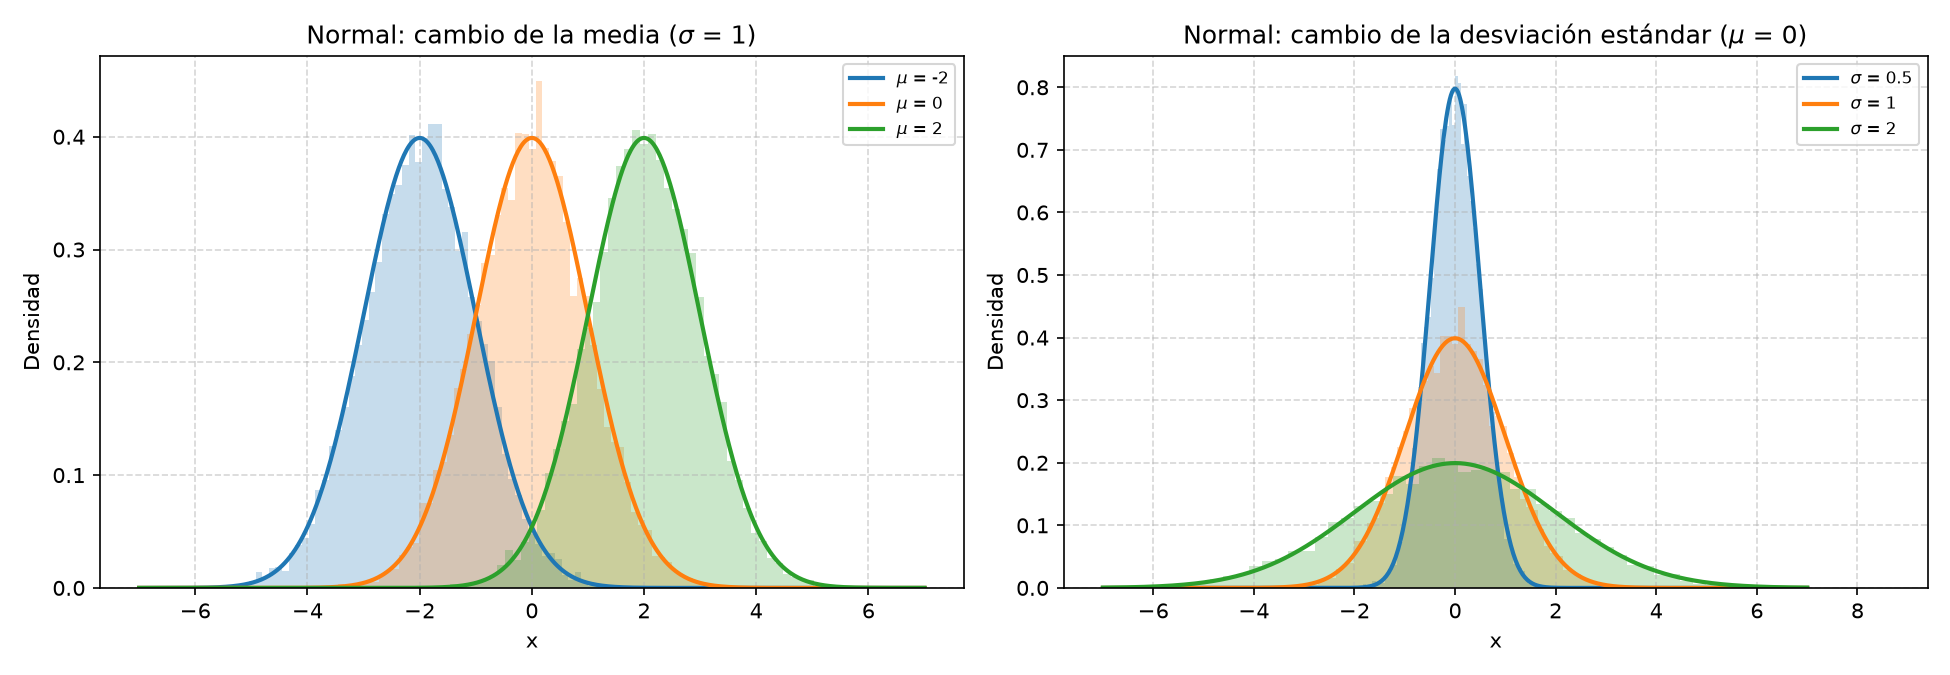
\includegraphics[width=\textwidth]{img/normal_parametros.png}
\caption{Distribución normal. Izquierda: cambio de la media con $\sigma = 1$. Derecha: cambio de la desviación estándar con $\mu = 0$. Histogramas de 10\,000 valores y densidad teórica.}
\label{fig:normal}
\end{figure}

\begin{figure}[htbp]
\centering
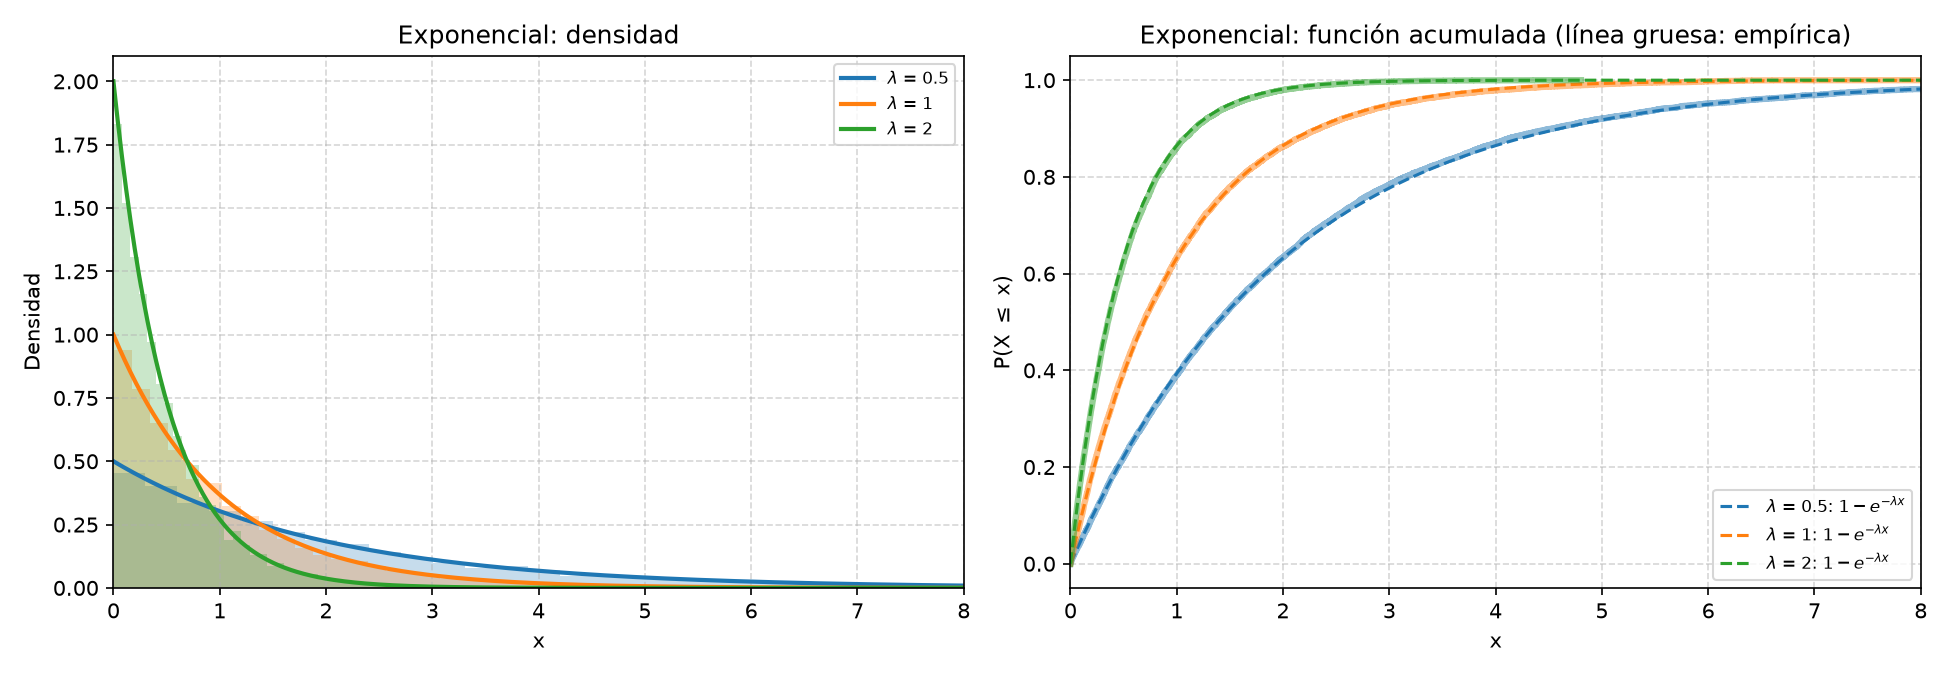
\includegraphics[width=\textwidth]{img/exponencial.png}
\caption{Distribución exponencial con $\lambda = 0.5, 1$ y $2$. Izquierda: densidad. Derecha: función acumulada empírica (línea gruesa) y teórica (línea discontinua).}
\label{fig:exponencial}
\end{figure}

\begin{figure}[htbp]
\centering
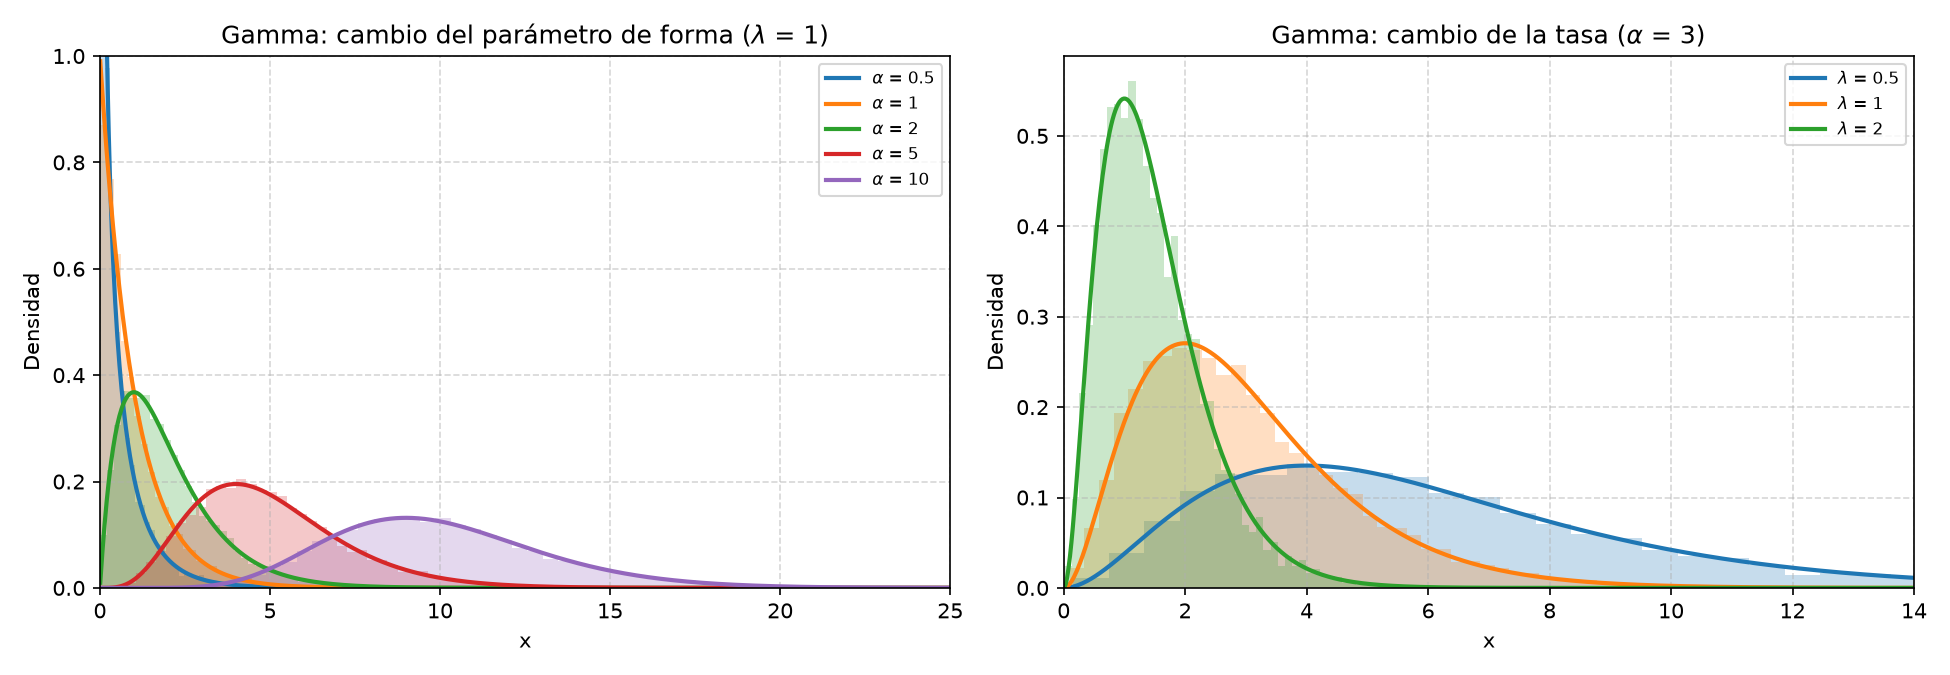
\includegraphics[width=\textwidth]{img/gamma.png}
\caption{Distribución gamma. Izquierda: cambio del parámetro de forma $\alpha$ con $\lambda = 1$. Derecha: cambio de la tasa $\lambda$ con $\alpha = 3$.}
\label{fig:gamma}
\end{figure}

\begin{itemize}
    \item \textbf{Normal.} En la Figura~\ref{fig:normal} (izquierda), cambiar $\mu$ desplaza la campana sin modificar su forma: las tres curvas tienen la misma altura y el mismo ancho. A la derecha, aumentar $\sigma$ de 0.5 a 2 ensancha la campana y baja su pico, de 0.80 a 0.20, porque el área bajo la curva debe seguir siendo 1.
    \item \textbf{Exponencial.} En la Figura~\ref{fig:exponencial}, $\lambda$ es a la vez la altura inicial de la densidad ($f(0) = \lambda$) y la rapidez con la que decrece: con $\lambda = 2$ casi toda la masa está por debajo de 2, y con $\lambda = 0.5$ la cola llega a más de 8. La acumulada empírica se superpone a la teórica.
    \item \textbf{Gamma, parámetro de forma.} En la Figura~\ref{fig:gamma} (izquierda), con $\alpha < 1$ la densidad es infinita en 0 y decrece; con $\alpha = 1$ es una exponencial; con $\alpha > 1$ aparece un máximo en $(\alpha - 1)/\lambda$ que se desplaza a la derecha, y la curva se vuelve más ancha y más simétrica al crecer $\alpha$.
    \item \textbf{Gamma, tasa.} En la Figura~\ref{fig:gamma} (derecha), $\lambda$ cambia la escala: con $\lambda = 2$ la densidad se comprime hacia 0 y es más alta, y con $\lambda = 0.5$ se estira. La forma es la misma y solo cambia la unidad de medida, como indica el documento fuente.
\end{itemize}

\subsection{Tarea 3: Análisis comparativo}

\begin{consola}[label=out:t3a]{Ejecución de \texttt{act11.py}: Tarea 3a}
=== Tarea 3a: momentos teóricos (t.) y de la muestra (m.); curtosis en exceso ===
              Caso  Media t.  Media m.  Desv. t.  Desv. m.  Asim. t.  Asim. m.  Curt. t.  Curt. m.
 Normal mu=-2, s=1      -2.0    -1.986     1.000     1.002     0.000    -0.023       0.0     0.012
  Normal mu=0, s=1       0.0    -0.009     1.000     0.994     0.000     0.009       0.0    -0.012
  Normal mu=2, s=1       2.0     2.004     1.000     0.998     0.000    -0.066       0.0     0.062
Normal mu=0, s=0.5       0.0    -0.003     0.500     0.502     0.000    -0.015       0.0    -0.048
  Normal mu=0, s=2       0.0    -0.018     2.000     2.003     0.000    -0.013       0.0    -0.070
 Exponencial l=0.5       2.0     1.985     2.000     1.977     2.000     1.992       6.0     5.692
   Exponencial l=1       1.0     1.005     1.000     1.019     2.000     1.962       6.0     5.224
   Exponencial l=2       0.5     0.511     0.500     0.513     2.000     2.015       6.0     5.940
  Gamma a=0.5, l=1       0.5     0.512     0.707     0.728     2.828     2.946      12.0    13.567
    Gamma a=1, l=1       1.0     1.019     1.000     1.040     2.000     2.136       6.0     7.077
    Gamma a=2, l=1       2.0     1.996     1.414     1.397     1.414     1.377       3.0     2.808
    Gamma a=5, l=1       5.0     5.002     2.236     2.214     0.894     0.897       1.2     1.307
   Gamma a=10, l=1      10.0    10.014     3.162     3.177     0.632     0.647       0.6     0.638
  Gamma a=3, l=0.5       6.0     5.938     3.464     3.410     1.155     1.178       2.0     2.377
    Gamma a=3, l=1       3.0     3.001     1.732     1.752     1.155     1.131       2.0     1.808
    Gamma a=3, l=2       1.5     1.488     0.866     0.860     1.155     1.153       2.0     1.993
\end{consola}

Las asimetrías y curtosis muestrales siguen a las teóricas. La normal tiene asimetría y curtosis en exceso cercanas a 0; la exponencial tiene asimetría 2 en teoría (1.99, 1.96 y 2.02 en las muestras) y curtosis 6; en la gamma la asimetría $2/\sqrt{\alpha}$ baja de 2.83 con $\alpha = 0.5$ a 0.63 con $\alpha = 10$, y la muestra da 2.95 y 0.65. La curtosis muestral es más ruidosa que las demás medidas, porque depende de las colas: por ejemplo, 5.22 contra 6 para la exponencial con $\lambda = 1$.

\begin{consola}[label=out:t3b]{Ejecución de \texttt{act11.py}: Tarea 3b}
=== Tarea 3b: P(a < X <= b), teórica y simulada ===
             Caso     Intervalo  P teórica  Proporción simulada  Diferencia  Error estándar
 Normal mu=0, s=1 (-1.96, 1.96]     0.9500               0.9520      0.0020          0.0022
 Normal mu=0, s=2       (-2, 2]     0.6827               0.6806     -0.0021          0.0047
Exponencial l=0.5        (0, 2]     0.6321               0.6335      0.0014          0.0048
  Exponencial l=2      (0, 0.5]     0.6321               0.6239     -0.0082          0.0048
   Gamma a=3, l=1        (2, 4]     0.4386               0.4269     -0.0117          0.0050
  Gamma a=10, l=1       (8, 12]     0.4742               0.4764      0.0022          0.0050
\end{consola}

Las proporciones simuladas están cerca de las probabilidades teóricas. Cinco de las seis diferencias están dentro de 1.7 errores estándar; la excepción es la gamma con $\alpha = 3$ y $\lambda = 1$ en el intervalo $(2, 4]$, con $-0.0117$, es decir 2.3 errores estándar. Con seis intervalos una diferencia de ese tamaño es posible por azar, y la prueba de la siguiente tabla no rechaza esa muestra.

\begin{consola}[label=out:t3c]{Ejecución de \texttt{act11.py}: Tarea 3c}
=== Tarea 3c: prueba de Kolmogorov-Smirnov contra la distribución teórica ===
              Caso      D  p-valor
 Normal mu=-2, s=1 0.0120   0.1107
  Normal mu=0, s=1 0.0107   0.2031
  Normal mu=2, s=1 0.0095   0.3213
Normal mu=0, s=0.5 0.0067   0.7513
  Normal mu=0, s=2 0.0065   0.7946
 Exponencial l=0.5 0.0085   0.4702
   Exponencial l=1 0.0072   0.6728
   Exponencial l=2 0.0103   0.2396
  Gamma a=0.5, l=1 0.0118   0.1217
    Gamma a=1, l=1 0.0092   0.3685
    Gamma a=2, l=1 0.0051   0.9538
    Gamma a=5, l=1 0.0094   0.3363
   Gamma a=10, l=1 0.0057   0.9038
  Gamma a=3, l=0.5 0.0100   0.2687
    Gamma a=3, l=1 0.0098   0.2932
    Gamma a=3, l=2 0.0108   0.1949
Rechazos al nivel 0.05: 0 de 16
\end{consola}

La prueba de Kolmogorov-Smirnov no rechaza ninguna de las 16 muestras al nivel de 0.05: los $p$-valores van de 0.11 a 0.95. Es decir, ninguna muestra es distinguible de su distribución teórica, lo que confirma que los parámetros se pasaron correctamente (en particular, la escala $1/\lambda$ en la exponencial y la gamma).

\begin{consola}[label=out:t3d]{Ejecución de \texttt{act11.py}: Tarea 3d}
=== Tarea 3d: relaciones entre las distribuciones ===
Gamma(alpha=1, lambda=1) contra Exponencial(1): D = 0.0092, p = 0.3685
Exponencial desde cero (lambda=2):        D = 0.0105, p = 0.2143
Gamma desde cero, suma de 3 exp. (l=2):   D = 0.0067, p = 0.7533
Mediana exponencial lambda=0.5: teórica ln2/lambda = 1.386, muestra = 1.388
Mediana exponencial lambda=1: teórica ln2/lambda = 0.693, muestra = 0.687
Mediana exponencial lambda=2: teórica ln2/lambda = 0.347, muestra = 0.353
Falta de memoria (lambda=1, s=1, t=1): P(X > 2 | X > 1) = 0.3744, P(X > 1) = 0.3673, teórica e^(-1) = 0.3679

Asimetría de la gamma al aumentar alpha:
 alpha  Asimetría teórica 2/raíz(alpha)  Asimetría muestral
     1                            2.000               1.975
     5                            0.894               0.895
    20                            0.447               0.456
   100                            0.200               0.165
\end{consola}

\begin{figure}[htbp]
\centering
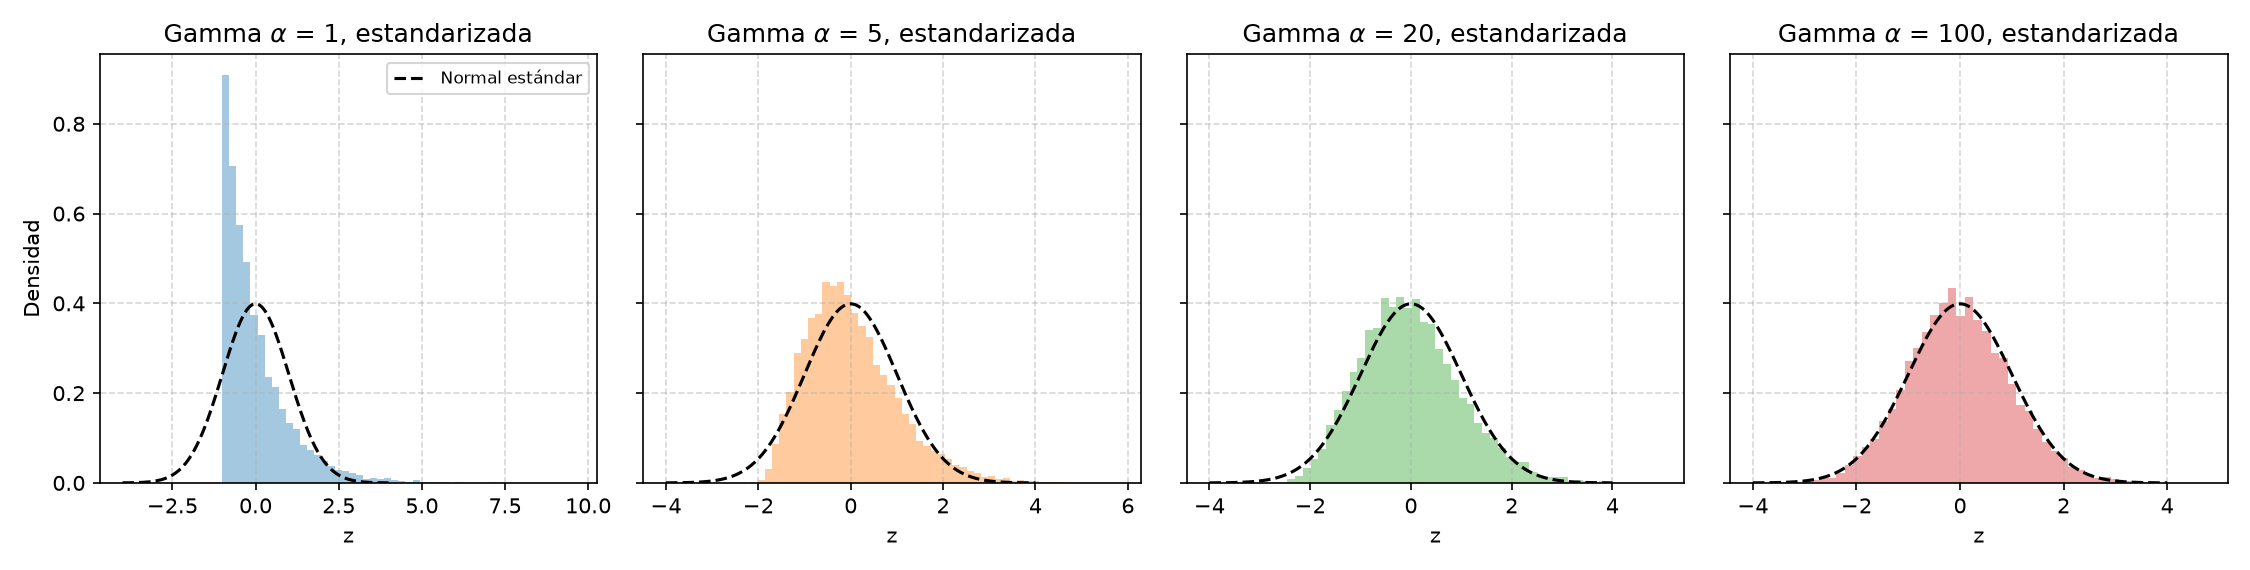
\includegraphics[width=\textwidth]{img/gamma_hacia_normal.png}
\caption{Muestras de una gamma con $\lambda = 1$ y $\alpha = 1, 5, 20$ y $100$, estandarizadas ($z = (x - \alpha)/\sqrt{\alpha}$), contra la densidad normal estándar.}
\label{fig:gamma_normal}
\end{figure}

\begin{itemize}
    \item \textbf{Gamma con $\alpha = 1$ es la exponencial.} La muestra de la gamma con $\alpha = 1$ no se distingue de una exponencial con $\lambda = 1$ ($D = 0.0092$, $p = 0.37$).
    \item \textbf{Los simuladores del documento fuente son correctos.} La exponencial por transformada inversa y la gamma como suma de tres exponenciales no se distinguen de sus distribuciones teóricas ($p = 0.21$ y $p = 0.75$).
    \item \textbf{Mediana.} Las medianas de la exponencial (1.388, 0.687 y 0.353) coinciden con $\ln 2/\lambda$ (1.386, 0.693 y 0.347), y son menores que las medias porque la distribución es asimétrica a la derecha.
    \item \textbf{Falta de memoria.} Entre los valores que ya superaron 1, la proporción que supera 2 es 0.3744, muy cercana a $P(X > 1) = 0.3673$ y a $e^{-1} = 0.3679$: haber esperado ya un tiempo no cambia la distribución del tiempo restante.
    \item \textbf{La gamma tiende a la normal.} En la Figura~\ref{fig:gamma_normal}, la gamma estandarizada es muy asimétrica con $\alpha = 1$ y casi indistinguible de la normal con $\alpha = 100$. La asimetría muestral baja de 1.975 a 0.165, siguiendo $2/\sqrt{\alpha}$ (de 2 a 0.2). Es consistente con el teorema central del límite, porque una gamma con $\alpha$ entero es una suma de $\alpha$ exponenciales.
\end{itemize}

\subsection{Tarea 4: Aplicación práctica}

\begin{consola}[label=out:t4]{Ejecución de \texttt{act11.py}: Tarea 4}
=== Tarea 4: aplicaciones prácticas (100000 simulaciones por situación) ===
1) Estatura ~ Normal(170, 7):
   P(165 < X < 180): teórica = 0.6859, simulada = 0.6863
   Estatura que supera el 95 % de la población: teórica = 181.51 cm, simulada = 181.47 cm
2) Tiempo entre llegadas ~ Exponencial(lambda = 3 por hora):
   Tiempo medio: teórico = 20.0 min, simulado = 20.09 min
   P(esperar más de 30 min): teórica = 0.2231, simulada = 0.2241
3) Tiempo hasta la llegada del 3.er cliente ~ Gamma(alpha = 3, lambda = 3 por hora):
   Tiempo medio: teórico = 60.0 min, simulado = 60.01 min
   P(tardar menos de 1 hora): teórica = 0.5768, simulada = 0.5760
\end{consola}

\begin{figure}[htbp]
\centering
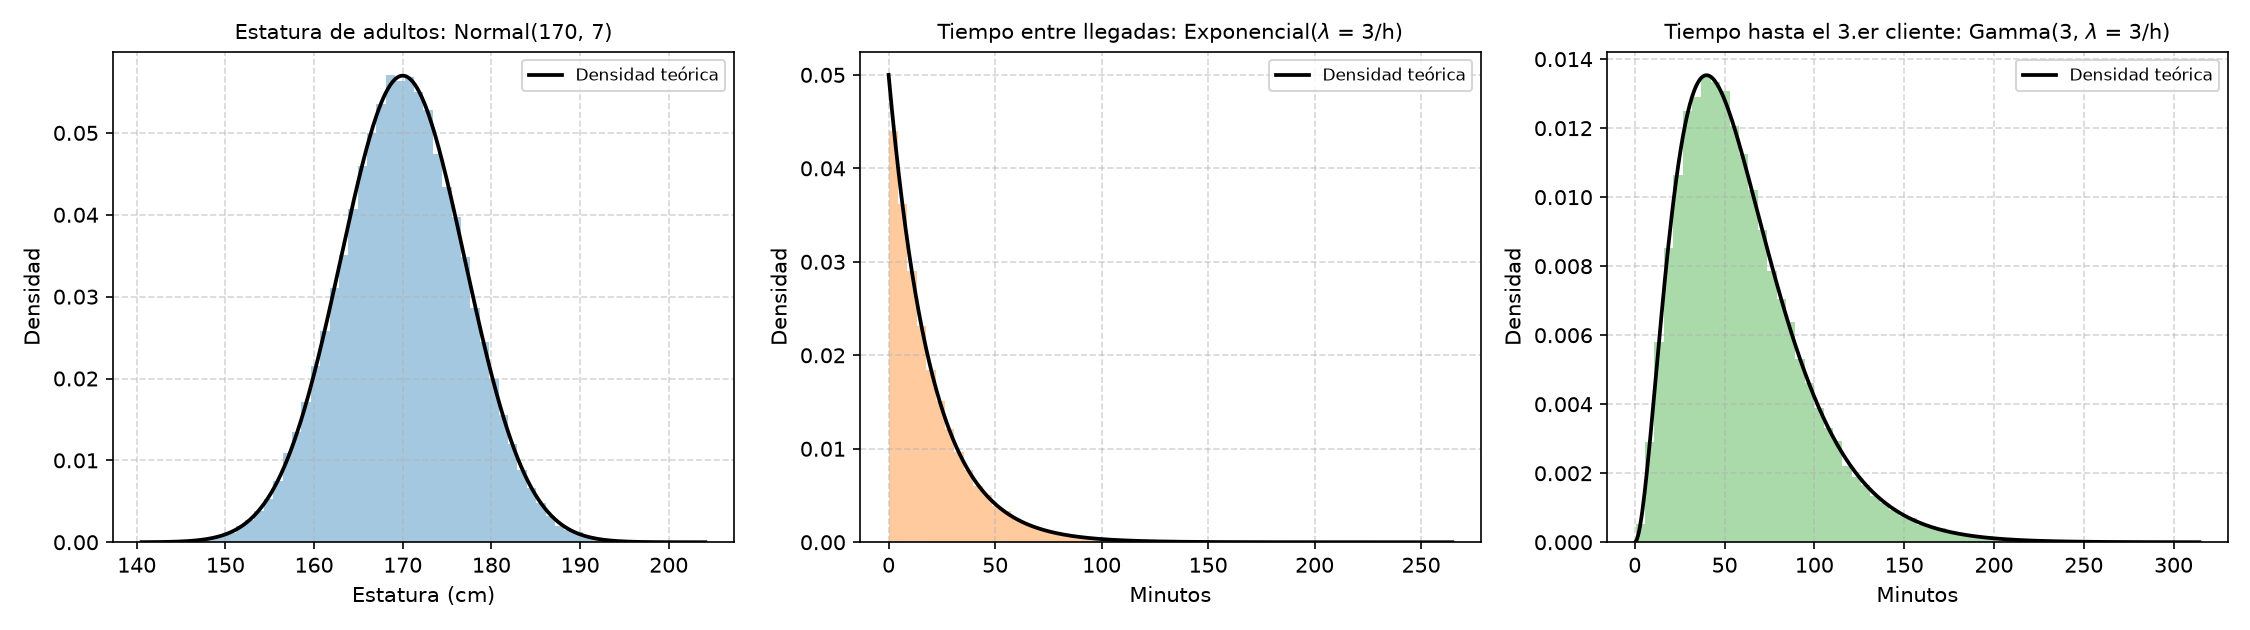
\includegraphics[width=\textwidth]{img/aplicaciones.png}
\caption{Tres aplicaciones: estatura de adultos (normal), tiempo entre llegadas (exponencial) y tiempo hasta el tercer cliente (gamma). Histogramas de 100\,000 valores simulados y densidad teórica.}
\label{fig:aplicaciones}
\end{figure}

La Tabla~\ref{tab:aplicaciones} resume cada situación y por qué la distribución es adecuada, y la Figura~\ref{fig:aplicaciones} muestra que los datos simulados siguen la densidad teórica.

\begin{table}[htbp]
\centering
\caption{Situaciones reales y distribución adecuada.}
\label{tab:aplicaciones}
\footnotesize
\renewcommand{\arraystretch}{1.3}
\begin{tabular}{p{2.3cm}p{5.2cm}p{5.4cm}}
\hline
\textbf{Distribución} & \textbf{Situación} & \textbf{Por qué es adecuada} \\
\hline
Normal & Estatura de adultos con media 170 cm y desviación 7 cm. La probabilidad de medir entre 165 y 180 cm es 0.686, y el 95\,\% mide menos de 181.5 cm. También los errores de medición de un instrumento \parencite{tecnm2026_documento_fuente}. & La estatura y el error resultan de la suma de muchos efectos pequeños e independientes, por lo que el teorema central del límite justifica una distribución simétrica en forma de campana. \\
Exponencial & Tiempo entre llegadas de clientes, con 3 llegadas por hora en promedio ($\lambda = 3$ por hora). El tiempo medio es 20 min y la probabilidad de esperar más de 30 min es 0.223. & Es el tiempo entre eventos que ocurren de forma independiente y a una tasa constante (proceso de Poisson), y su falta de memoria significa que haber esperado ya no cambia lo que falta \parencite{tecnm2026_documento_fuente}. \\
Gamma & Tiempo hasta la llegada del tercer cliente con la misma tasa ($\alpha = 3$, $\lambda = 3$ por hora). El tiempo medio es 60 min y la probabilidad de que lleguen tres en menos de una hora es 0.577. & Es la suma de $\alpha$ tiempos exponenciales independientes: el tiempo hasta el $\alpha$-ésimo evento. \\
\hline
\end{tabular}
\end{table}

\section{Conclusiones}

Las tres distribuciones continuas se simularon con \texttt{numpy} y en todos los casos las muestras coincidieron con la teoría: las medias, desviaciones estándar y asimetrías estuvieron cerca de los valores teóricos, las proporciones de los intervalos coincidieron con las calculadas con la función acumulada, y la prueba de Kolmogorov-Smirnov no rechazó ninguna de las 16 muestras. Un detalle práctico que esto confirmó es que, con la parametrización del documento fuente, \texttt{numpy} y \texttt{scipy} necesitan la escala $1/\lambda$ en lugar de $\lambda$; con la escala equivocada las muestras habrían salido con la media incorrecta.

El efecto de los parámetros es distinto en cada distribución. En la normal, la media desplaza la curva y la desviación estándar controla su ancho y, por tanto, su altura. En la exponencial, $\lambda$ determina la rapidez del decaimiento. En la gamma, $\alpha$ cambia la forma, desde una curva infinita en 0 hasta una casi normal, y $\lambda$ solo cambia la escala. Las tres están relacionadas: la gamma con $\alpha = 1$ es una exponencial, la gamma con $\alpha$ entero es la suma de exponenciales y, al crecer $\alpha$, se acerca a la normal. En las aplicaciones, la elección de la distribución depende del fenómeno: la normal para cantidades que resultan de muchos efectos pequeños, la exponencial para el tiempo de espera hasta un evento y la gamma para el tiempo hasta el $\alpha$-ésimo evento.

\referencias

\end{document}
